%!TEX root = ../thesis.tex
%*******************************************************************************
%****************************** Third Chapter **********************************
%*******************************************************************************
\chapter{Design}
\graphicspath{{Chapter5/Figs/Raster/}{Chapter5/Figs/}}

Following the discussion in Chapter 2.3.1 and 2.5, the designs for this project 
will be created with a public permissioned blockchain based on Hyperledger Fabric in mind.
It has become clear that a blockchain specific, high-fidelity prototyping tool is needed 
to create system designs such as data and transaction models.

\section*{Hyperledger Composer}

Hyperledger Composer is an open source development toolset and framework that aims to 
accelerate time to value for blockchain projects. It offers business-centric 
abstractions, allowing business owners and developers to rapidly develop 
use cases and model a blockchain network. The design tools offered take the forms of:
\begin{itemize}
    \setlength\itemsep{0em}            
    \item a .cto file to define data models for assets, participants and transactions
    \item a .js file to define logic (code) for smart contracts triggered by transactions
    \item a .acl file to define access control rules for assets, participants and transactions\\
    \citep{official2018composer}
\end{itemize}

See figure \ref{fig:composer2fabric} for a visual explainer of how Hyperledger Composer 
helps designers and developers create these high level definitions.

\begin{figure}[!h] 
    \centering    
    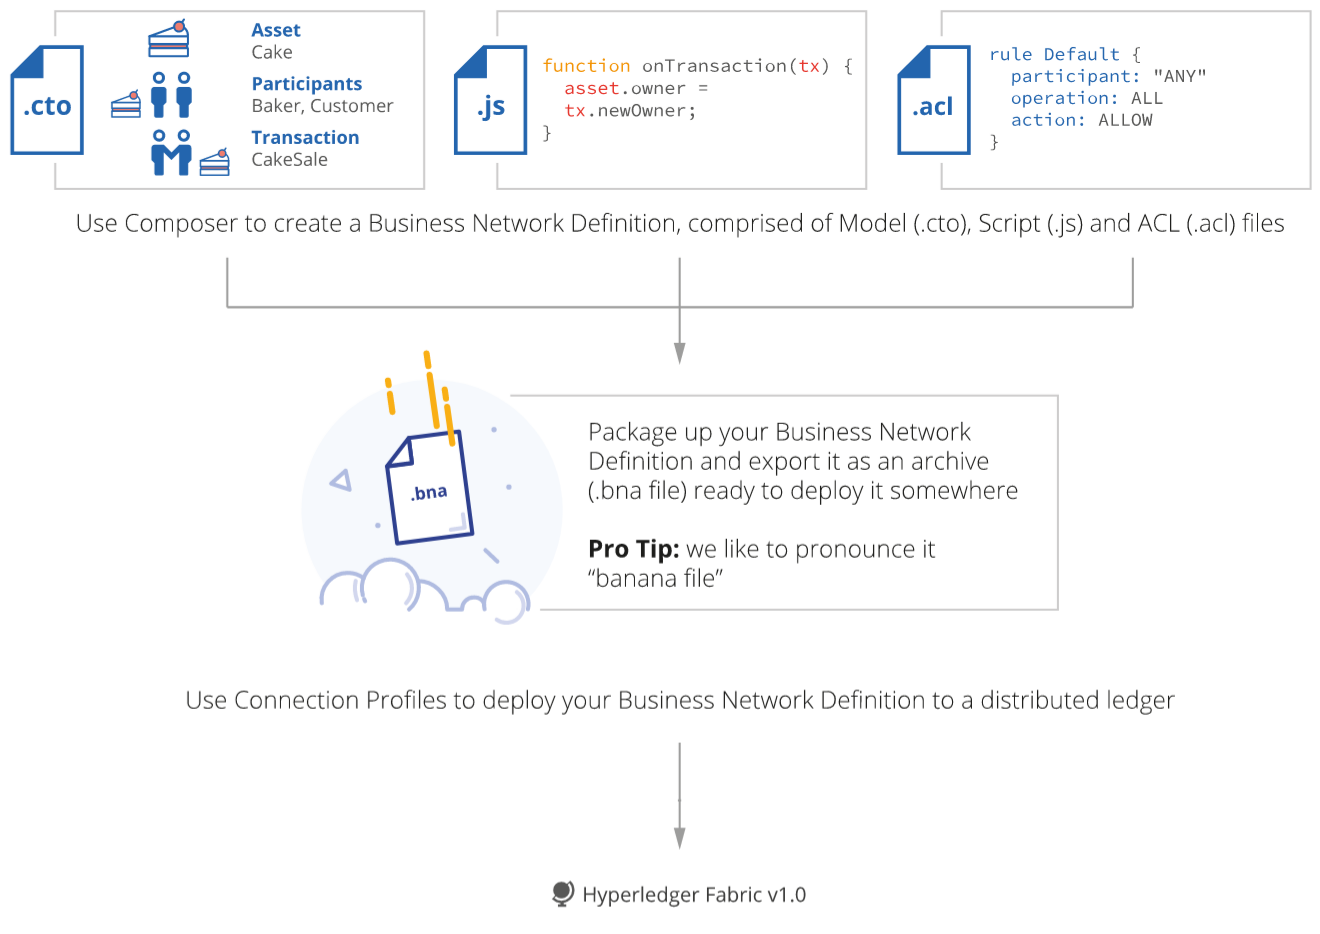
\includegraphics[width=1.0\textwidth]{composer2fabric}
    \caption[Hyperledger Composer]
        {Components in the Hyperledger Composer framework and how it deploys to 
        Hyperledger Fabric \citep{cuicapuza2017composer}}
    \label{fig:composer2fabric}
\end{figure}
% https://medium.com/@RichardCuica/hyperledgers-fabric-composer-simplifying-business-networks-on-blockchain-94313b979671

A significant advantage of using Hyperledger Composer is its ability to package these 
prototype definitions and deploy it to Hyperledger Fabric, our target blockchain platform. 
This will speed up the implementation of the proposed demonstrator applications 
in the next stage.

Throughout the design process, the hyperledger composer notations are converted into class 
diagrams and activity diagrams with PlantUML, an open source language-to-diagram drawing tool.

The discussion below may regularly refer back to the functional requirements (FR) and 
non-functional requirements (NR) defined in the previous Chapter 4.

\section{Participants, Assets and Transactions in the Blockchain Network}

\subsection{Use Cases}

automatic formative assessments Annette's student

schema --> reviewer

\subsection{Access and Permissions on Assets}
Role based and attribute based

\section{Logic and Events in Smart Contracts}

\section{Limitations}
No institutional approvers for certificates
No different tiers of privileges for teachers for roles such as module leader, module reviewer, supporting staff

\section{User Interfaces for Client Applications}
